% https://tex.stackexchange.com/a/762421
% to obtain the correct Brunnian or Borromean knot, the following rules must hold: (e1) Blue always goes over Green and under Red; (e2) Green always goes over Red and under Blue; (e3) Red always goes over Blue and under Green.
\documentclass[tikz,border=5mm]{standalone}
\usetikzlibrary{knots}

\begin{document}
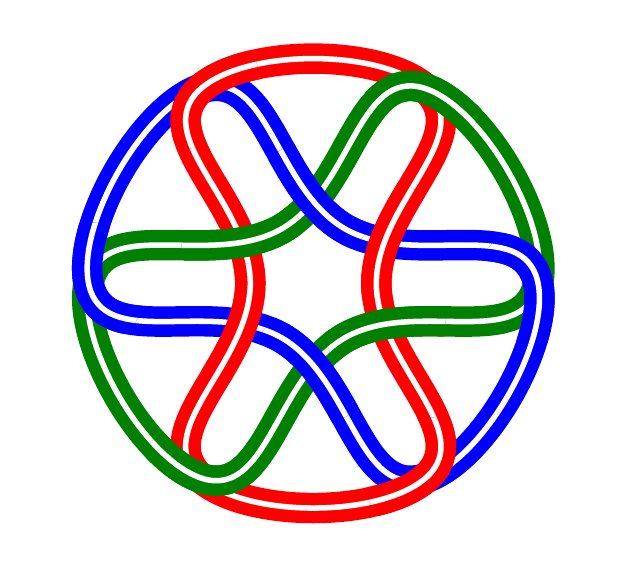
\begin{tikzpicture}
  \tikzset{
    vespa ring/.style={
      draw=#1, 
      line width=4.5pt, 
      line join=round
      double=white,
      double distance=2pt,
    },
    vespa ring/.default=red,
  }
  \newcommand{\vespawaist}[1]{
    (#1:0.8)
    .. controls (51+#1:1.28) and (42+#1:2.69) .. (58+#1:2.83) % Ombro
    .. controls (72+#1:3.16) and (108+#1:3.16) .. (122+#1:2.83) % Topo elevado
    .. controls (138+#1:2.69) and (129+#1:1.28) .. (180+#1:0.8) % Cintura esquerda
    .. controls (-129+#1:1.28) and (-138+#1:2.69) .. (-122+#1:2.83) % Ombro inferior
    .. controls (-108+#1:3.16) and (-72+#1:3.16) .. (-58+#1:2.83) % Base elevada
    .. controls (-42+#1:2.69) and (-51+#1:1.28) ..
    cycle
  }

  \begin{knot}[
        % draft mode=crossings,
        clip radius=20pt,
        background color=white,
    ]
    \strand [
      only when rendering/.style={vespa ring},
    ] (0,0) \vespawaist{0};
    \strand [
      only when rendering/.style={vespa ring=blue},
    ] (0,0) \vespawaist{60};
    \strand [
      only when rendering/.style={vespa ring=green!50!black},
    ] (0,0) \vespawaist{120};
    \flipcrossings{5,6,7,8,}
  \end{knot}
\end{tikzpicture}
\end{document}
